	\section{Introduction}


    \begin{frame}{Introducing myself}
        \begin{columns}
            % Column 1
            \begin{column}{0.5\textwidth}
                \begin{itemize}
                    \item Isak Hammer, 27 year old, Lofoten
                    \item Graduate student in Industrial Mathematics
                    \item Research Focus: Analysis and numerical techniques for Partial Differential Equations (PDEs), with a strong emphasis on applications for Finite Element Methods (FEM).
                \end{itemize}
            \end{column}

            % Column 2
            \begin{column}{0.5\textwidth}
                \begin{figure}
                    \centering
                    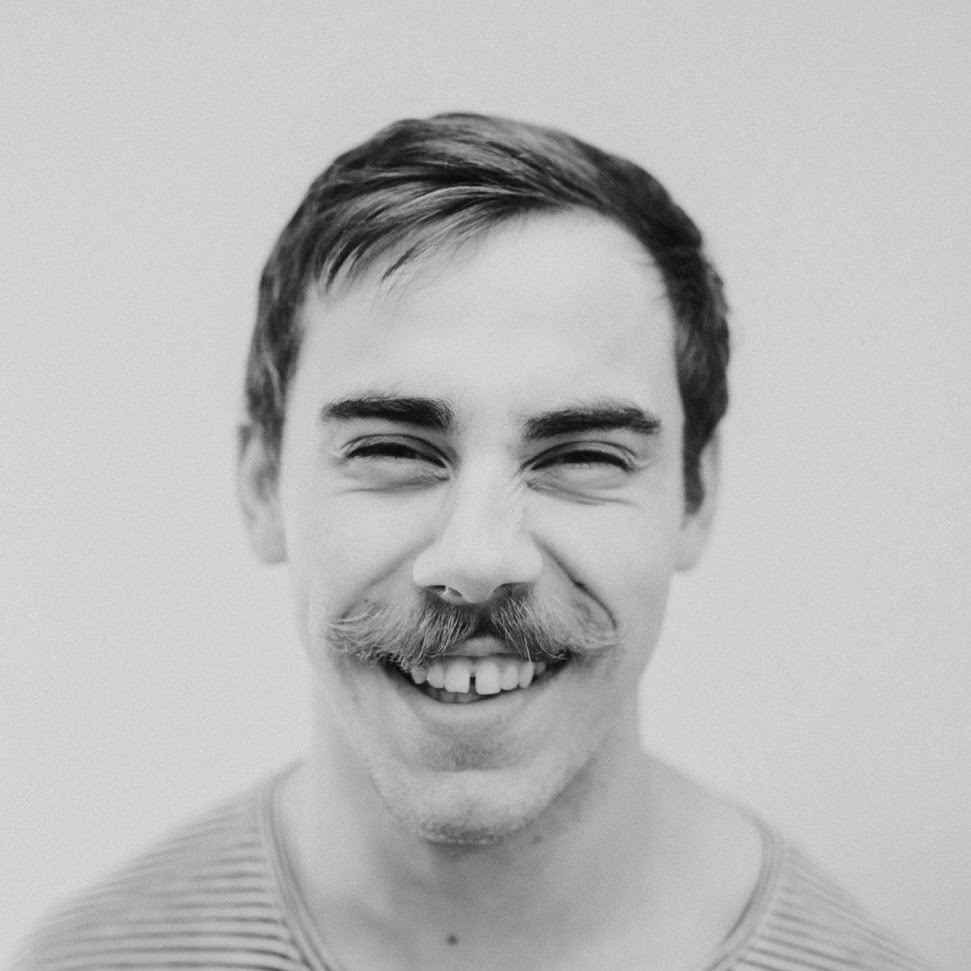
\includegraphics[width=0.7\textwidth]{figures/isak.jpg}
                \end{figure}
            \end{column}
        \end{columns}
    \end{frame}

\begin{frame}{Importance and Motivation of the Cahn Hilliard Equation}
    \begin{columns}
        % Column 1
        \begin{column}{0.5\textwidth}
            \begin{itemize}
                \item Modelling two-component phase separation of liquids\footnotemark.
                \item Modelling of so-called lipid rafts in biological membrane dynamics \footnotemark.
            \end{itemize}
        \end{column}
        \begin{column}{0.5\textwidth}
            \begin{itemize}
                \item Droplet dynamics, i.e., coalescence, breakup and movement by coupling with Navier-Stokes \footnotemark.
            \end{itemize}
        \end{column}
    \end{columns}
    \footnotetext[1]{\fullcite{cahn1959free}}
    \footnotetext[2]{\fullcite{yushutin2019computational}}
    \footnotetext[3]{\fullcite{zimmermann2019calculation}}
\end{frame}
